\documentclass[serif,mathserif]{beamer}
%\documentclass[handout]{beamer}
\usepackage{amsmath, amsfonts, epsfig, xspace}
\usepackage{algorithm,algorithmic}
\usepackage{pstricks,pst-node}
\usepackage{multimedia}
\usepackage[normal,tight,center]{subfigure}
\setlength{\subfigcapskip}{-.5em}
%\usepackage{beamerthemesplit}
\usetheme{lankton-keynote}
\usepackage[utf8x]{inputenc}
\usepackage[T1]{fontenc}
\setbeamertemplate{footline}[frame number]

\author[Stefan Sobek]{Stefan Sobek}

\title[Masterarbeit\hspace{2em}\insertframenumber/\inserttotalframenumber]{Implementierung eines Webservices nach \\ ISO 29002-31
Query for characteristic data}

\date{11. Februar 2014} %leave out for today's date to be insterted

\institute{Fernuni Hagen \\ Fakultät für Mathematik und Informatik \\ Lehrgebiet Datenbanksysteme für neue Anwendungen}

\begin{document}

\maketitle

%\section{Introduction}  % add these to see outline in slides

\begin{frame}
  \frametitle{Überblick}
\begin{columns}
        \column{.50\textwidth}
 \begin{itemize}
  \item Aufgabenbeschreibung
    \begin{itemize}
    \item Problemstellung
    \item Lösungsoptionen
    \item Zielsetzung
    \item Gesamtkontext und Abgrenzung
    \item Datenflüsse
    \end{itemize}
  \item Anforderungsanalyse
    \begin{itemize}
    \item Analyse ISO 29002-31
    \item Analyse ISO 22745-30
    \item Use Cases
    \end{itemize}
    \item System- und Softwareentwurf
    \begin{itemize}
    \item Auswahlprozess
    \item Architektur\pause
    \end{itemize}
  \end{itemize}
  
     \column{.50\textwidth}
   \begin{itemize}  
     
   \item Implementierung
    \begin{itemize}
    \item Configuration Management
    \item Webservice
    \item Query Verarbeitung
    \item Transformation
    \item Fehlerbehandlung
    \item SOAP-Webservice
    \end{itemize}    
    \item Schlußfolgerung  
 \end{itemize}
\end{columns}
\end{frame}

\begin{frame}
  \frametitle{Problemstellung}
  Heutiger automatisierter Produktdatenaustausch\pause
  \begin{itemize}
  \item basiert auf Schemata\pause
  \item häufig ein starres Schema\pause
  \item dadurch oft unflexibel durch fest verdrahtetes Modell\pause 
  \item hat bei Anpassungen hohe Änderungskosten
  %leave out the \pause on the final item
  \end{itemize}
\end{frame}

%\section{Main Body} % add these to see outline in slides

\begin{frame}
  \frametitle{Lösung}
  Abfrage- und Antwortschnittstelle basierend auf Schemata\pause
  \begin{itemize}
  \item ist flexibel\pause
  \item einheitliches Schnittstelle\pause
  \item dadurch bei Einhaltung keine Änderungen nötwendig
  \end{itemize}
\end{frame}

\begin{frame}
  \frametitle{Lösung}
  Es bieten sich vorhande ISO-Standards für flexible Abfrage- und Antwortschnittstellen an, z.B.:\pause
  \begin{itemize}
  \item ISO 22745-35 - Open technical dictionaries and their application to master data: Query for characteristic data\pause
  \item ISO 29002-31 - Exchange of characteristic data: Query for characteristic data
  \end{itemize}
\end{frame}

\begin{frame}
  \frametitle{Zielsetzung}
  Implementierung einer flexiblen Abfrage- und Antwortschnittstelle \pause
  \begin{itemize}
  \item Analyse der ISO 29002-31 - Query for characteristic data\pause
     \begin{itemize}
     \item Betrachtung nach Möglichkeiten einer herkömmlichen SQL-Schnittstelle (Projektion, Selektion)\pause
     \item Aufsetzen von Use Cases\pause
     \end{itemize}
  \item Prototypische Implementierung basierend auf ISO 29002-31 - Query for characteristic data\pause
      \begin{itemize}
      \item Datenbasis PLIB Datenbank\pause
      \item Nutzung vorhandener Prozeduren der PLIB-Datenbank
      \end{itemize}
  \end{itemize}
\end{frame}

\begin{frame}
  \frametitle{Gesamtkontext und Abgrenzung}
    Abschlussarbeiten um die PLIB
  \begin{figure}[t]
    %\centering
    %\subfigure[First Frame]{
    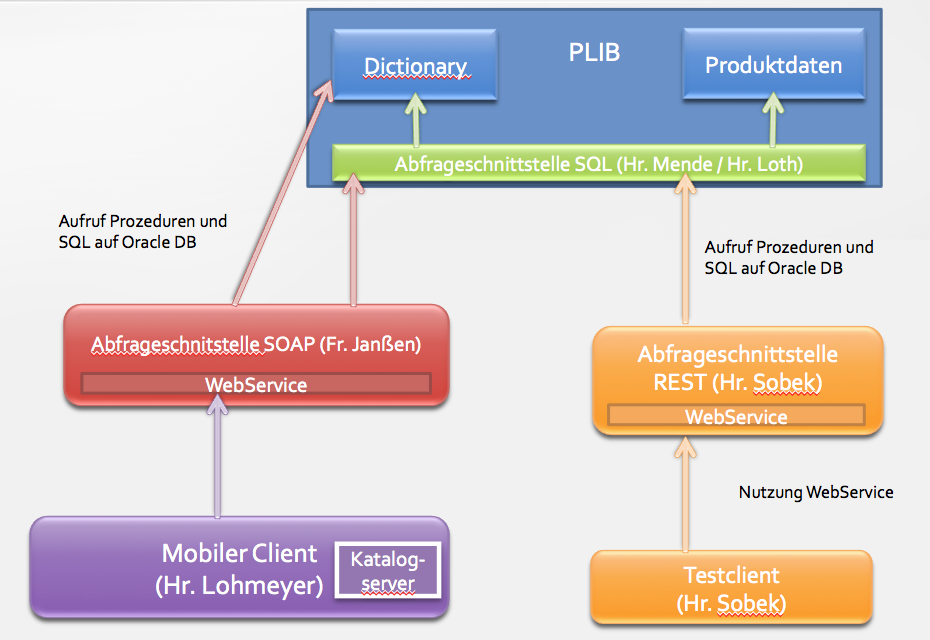
\includegraphics[width=7.5cm]{images/gesamtkontext_plib.png}
    %\subfigure[Middle Frame]{
    %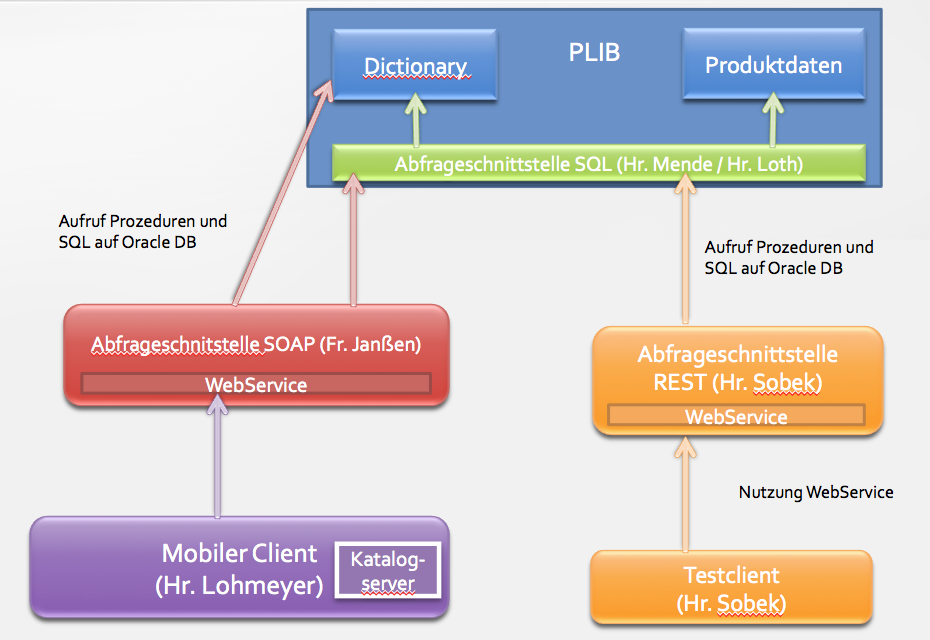
\includegraphics[width=3cm]{images/gesamtkontext_plib.png}}
    %\subfigure[Last Frame]{
    %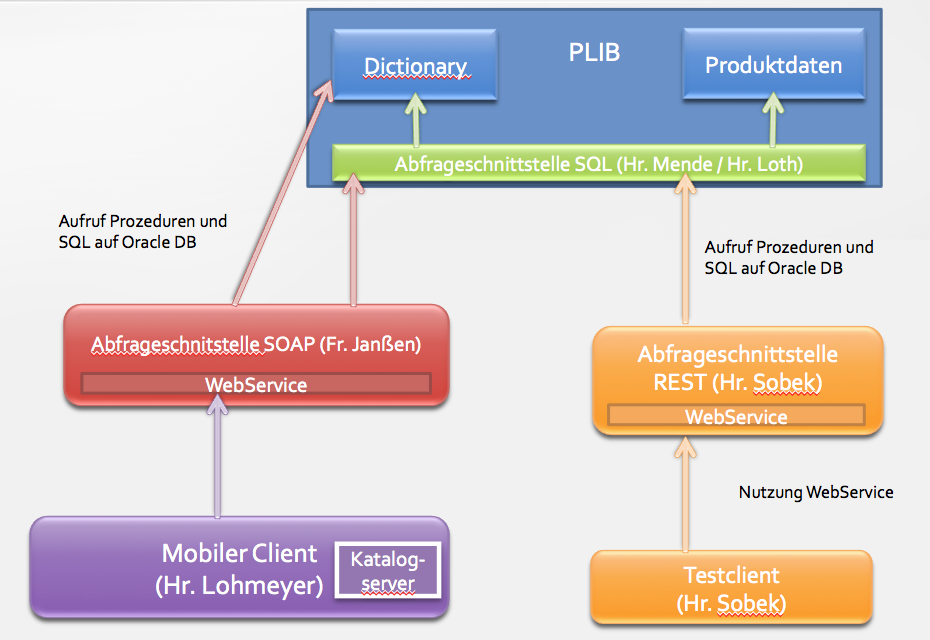
\includegraphics[width=3cm]{images/gesamtkontext_plib.png}}
  \end{figure}
\end{frame}

\begin{frame}
  \frametitle{Gesamtkontext und Abgrenzung}
    Abschlussarbeiten um die PLIB
  \begin{figure}[t]
    %\centering
    %\subfigure[First Frame]{
    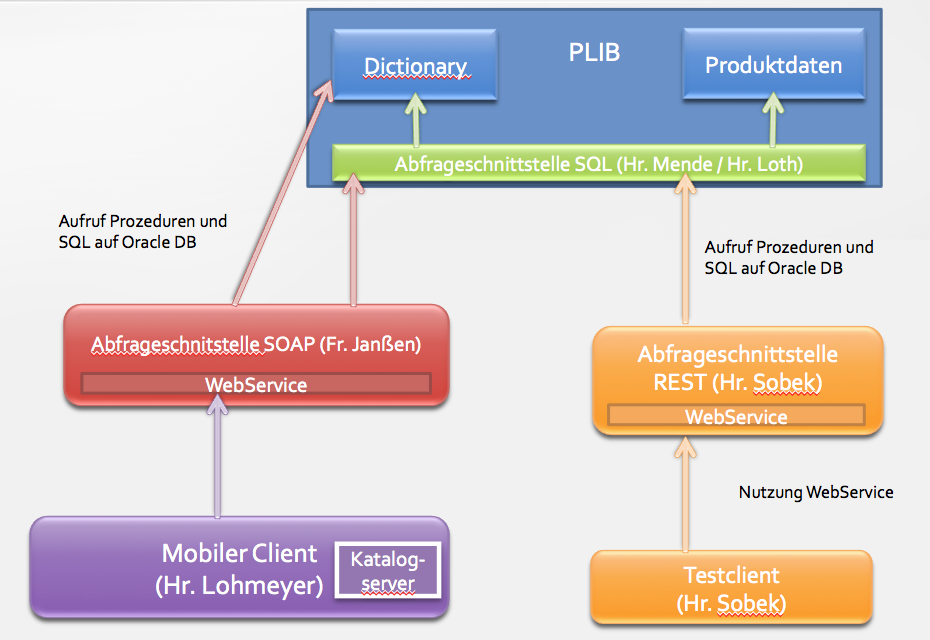
\includegraphics[width=7.5cm]{images/gesamtkontext_plib.png}
    %\subfigure[Middle Frame]{
    %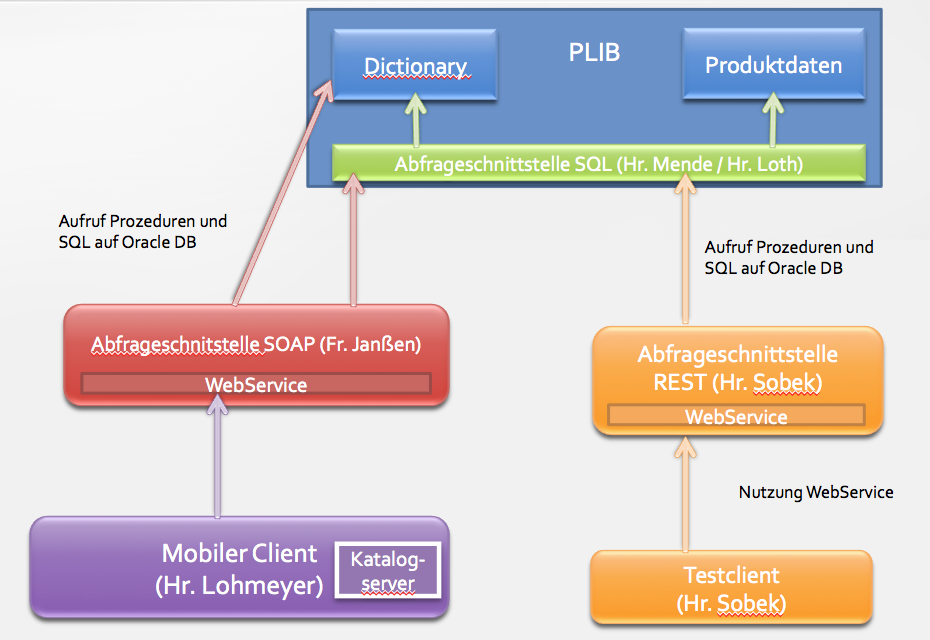
\includegraphics[width=3cm]{images/gesamtkontext_plib.png}}
    %\subfigure[Last Frame]{
    %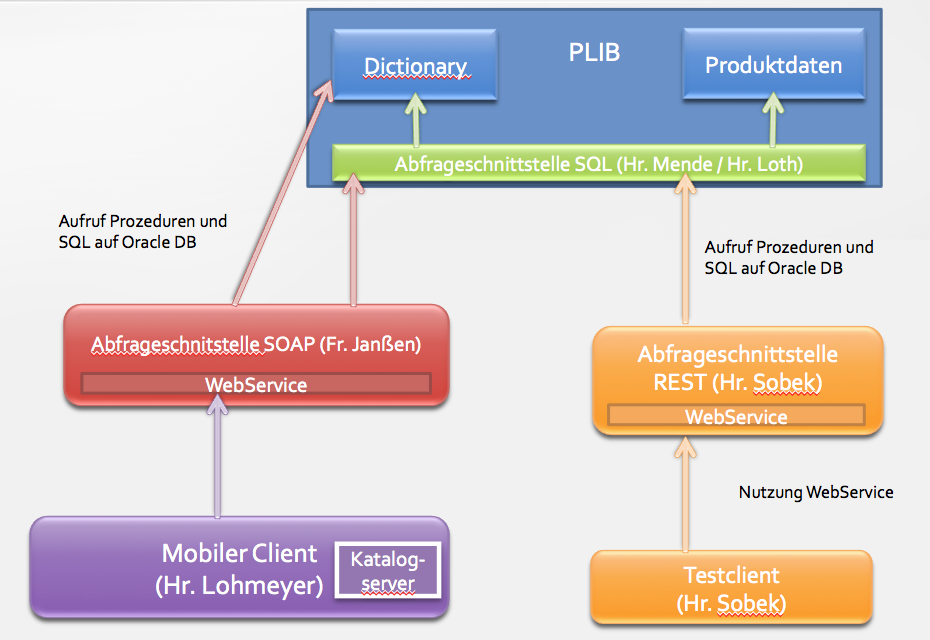
\includegraphics[width=3cm]{images/gesamtkontext_plib.png}}
  \end{figure}
\end{frame}

% \section{Conclusion} % add these to see outline in slides

\begin{frame}
  \frametitle{Credits}
  \begin{itemize}
  \item Brought to you by www.shawnlankton.com
  \item Please let me know about improvements!
  \item This was supposed to look like a KeyNote Show
  \item inspiration: http://www.ucl.ac.uk/~ucbpeal/latexposter.html
  \item inspiration: http://newsgroups.derkeiler.com/... (in code)
        %http://newsgroups.derkeiler.com/Archive/Comp/comp.text.tex/2007-11/msg00299.html
  \end{itemize}
\end{frame}

\begin{frame}
  \frametitle{Questions}
\end{frame}
\end{document}
